\documentclass{beamer}\usepackage[]{graphicx}\usepackage[]{graphicx}\usepackage[]{xcolor}
% maxwidth is the original width if it is less than linewidth
% otherwise use linewidth (to make sure the graphics do not exceed the margin)
\makeatletter
\def\maxwidth{ %
  \ifdim\Gin@nat@width>\linewidth
    \linewidth
  \else
    \Gin@nat@width
  \fi
}
\makeatother

\definecolor{fgcolor}{rgb}{0.345, 0.345, 0.345}
\newcommand{\hlnum}[1]{\textcolor[rgb]{0.686,0.059,0.569}{#1}}%
\newcommand{\hlstr}[1]{\textcolor[rgb]{0.192,0.494,0.8}{#1}}%
\newcommand{\hlcom}[1]{\textcolor[rgb]{0.678,0.584,0.686}{\textit{#1}}}%
\newcommand{\hlopt}[1]{\textcolor[rgb]{0,0,0}{#1}}%
\newcommand{\hlstd}[1]{\textcolor[rgb]{0.345,0.345,0.345}{#1}}%
\newcommand{\hlkwa}[1]{\textcolor[rgb]{0.161,0.373,0.58}{\textbf{#1}}}%
\newcommand{\hlkwb}[1]{\textcolor[rgb]{0.69,0.353,0.396}{#1}}%
\newcommand{\hlkwc}[1]{\textcolor[rgb]{0.333,0.667,0.333}{#1}}%
\newcommand{\hlkwd}[1]{\textcolor[rgb]{0.737,0.353,0.396}{\textbf{#1}}}%
\let\hlipl\hlkwb

\usepackage{framed}
\makeatletter
\newenvironment{kframe}{%
 \def\at@end@of@kframe{}%
 \ifinner\ifhmode%
  \def\at@end@of@kframe{\end{minipage}}%
  \begin{minipage}{\columnwidth}%
 \fi\fi%
 \def\FrameCommand##1{\hskip\@totalleftmargin \hskip-\fboxsep
 \colorbox{shadecolor}{##1}\hskip-\fboxsep
     % There is no \\@totalrightmargin, so:
     \hskip-\linewidth \hskip-\@totalleftmargin \hskip\columnwidth}%
 \MakeFramed {\advance\hsize-\width
   \@totalleftmargin\z@ \linewidth\hsize
   \@setminipage}}%
 {\par\unskip\endMakeFramed%
 \at@end@of@kframe}
\makeatother

\definecolor{shadecolor}{rgb}{.97, .97, .97}
\definecolor{messagecolor}{rgb}{0, 0, 0}
\definecolor{warningcolor}{rgb}{1, 0, 1}
\definecolor{errorcolor}{rgb}{1, 0, 0}
\newenvironment{knitrout}{}{} % an empty environment to be redefined in TeX

\usepackage{alltt}\usepackage[]{graphicx}\usepackage[]{xcolor}
% maxwidth is the original width if it is less than linewidth
% otherwise use linewidth (to make sure the graphics do not exceed the margin)
% \makeatletter
% \def\maxwidth{ %
%   \ifdim\Gin@nat@width>\linewidth
%     \linewidth
%   \else
%     \Gin@nat@width
%   \fi
% }
% \makeatother
% 
% 
% \definecolor{fgcolor}{rgb}{0.345, 0.345, 0.345}
% \newcommand{\hlnum}[1]{\textcolor[rgb]{0.686,0.059,0.569}{#1}}%
% \newcommand{\hlstr}[1]{\textcolor[rgb]{0.192,0.494,0.8}{#1}}%
% \newcommand{\hlcom}[1]{\textcolor[rgb]{0.678,0.584,0.686}{\textit{#1}}}%
% \newcommand{\hlopt}[1]{\textcolor[rgb]{0,0,0}{#1}}%
% \newcommand{\hlstd}[1]{\textcolor[rgb]{0.345,0.345,0.345}{#1}}%
% \newcommand{\hlkwa}[1]{\textcolor[rgb]{0.161,0.373,0.58}{\textbf{#1}}}%
% \newcommand{\hlkwb}[1]{\textcolor[rgb]{0.69,0.353,0.396}{#1}}%
% \newcommand{\hlkwc}[1]{\textcolor[rgb]{0.333,0.667,0.333}{#1}}%
% \newcommand{\hlkwd}[1]{\textcolor[rgb]{0.737,0.353,0.396}{\textbf{#1}}}%
% % \let\hlipl\hlkwb
% 
% \usepackage{framed}
% \makeatletter
% \newenvironment{kframe}{%
%  \def\at@end@of@kframe{}%
%  \ifinner\ifhmode%
%   \def\at@end@of@kframe{\end{minipage}}%
%   \begin{minipage}{\columnwidth}%
%  \fi\fi%
%  \def\FrameCommand##1{\hskip\@totalleftmargin \hskip-\fboxsep
%  \colorbox{shadecolor}{##1}\hskip-\fboxsep
%      % There is no \\@totalrightmargin, so:
%      \hskip-\linewidth \hskip-\@totalleftmargin \hskip\columnwidth}%
%  \MakeFramed {\advance\hsize-\width
%    \@totalleftmargin\z@ \linewidth\hsize
%    \@setminipage}}%
%  {\par\unskip\endMakeFramed%
%  \at@end@of@kframe}
% \makeatother
% 
% \definecolor{shadecolor}{rgb}{.97, .97, .97}
% \definecolor{messagecolor}{rgb}{0, 0, 0}
% \definecolor{warningcolor}{rgb}{1, 0, 1}
% \definecolor{errorcolor}{rgb}{1, 0, 0}
% \newenvironment{knitrout}{}{} % an empty environment to be redefined in TeX
% 
% \usepackage{alltt}					% Document class

\mode<presentation>
{
  \usetheme{default}                    % Set theme
  \usecolortheme{default}               % Set colors
  \usefonttheme{default}                % Set font theme
  \setbeamertemplate{caption}[numbered] % Set caption to be numbered
}

\usepackage{graphicx}  % For including figures
\usepackage{booktabs}  % For table rules
\usepackage{hyperref}  % For cross-referencing

\title{Introduction}  % Presentation title
\author{Andrew Ker}                              % Presentation author
\date{\today}
\IfFileExists{upquote.sty}{\usepackage{upquote}}{}
\IfFileExists{upquote.sty}{\usepackage{upquote}}{}
\begin{document}


% Title page
% This page includes the information defined earlier including
% title, author/s, affiliation/s and the date
\begin{frame}
  \titlepage
\end{frame}

% Outline
% This page includes the outline (Table of content) of the presentation.
% All sections and subsections will appear in the outline by default.
\begin{frame}{Outline}
  \tableofcontents
\end{frame}

% The following is the most frequently used slide types in beamer
% The slide structure is as follows:
%
%\begin{frame}{<slide-title>}
%	<content>
%\end{frame}

\section{Introduction}

\begin{frame}{Basic Information}
	Where I have Lived:
    \begin{itemize}
		\item I was originally born in Pomona, California. I lived in California for the first few years of my life
        \item My parents and I then moved to Casper, Wyoming, where we lived for 8 years.
          \item My family moved to Centennial, Colorado for a few years.
            \item We moved back to Casper, Wyoming before I started high school.
              \item For my first semester of college, I liven in Boulder, Colorado.
                \item I lived in Laramie, Wyoming for the remainder of Undergrad.
                  \item I now live in Lincoln, Nebraska!
	\end{itemize}
\end{frame}

\begin{frame}{Basic Information}
  \begin{itemize}
    \item My birthday is November 3rd
      \item I enjoy watching movies. I like to rate movies after I've seen them, and I try to branch out to see
      various types of movies
        \item I also enjoy sports. I love watching baseball, footbal, and basketball. I also play fantasy sports
        in my free time.
  \end{itemize}
\end{frame}

\begin{frame}{Basic Information: Program}
  \begin{itemize}
    \item I am currently in my first year of the graduate program in Statistics at UNL.
      \item I am also working as a TA within the Department of Statistics at UNL.
        \item I anticipate getting a Master's, but I'm not sure about the PhD.
        \begin{itemize}
          \item If I get the Master's, my anticipated graduation date is May 2024.
            \item If I go for the PhD, my anticipated graduation date is around May 2027ish.
        \end{itemize}
          \item I'm not exactly sure what I want to do, but I enjoy sports analytics, Bayesian statistics, and time series analysis right now
  \end{itemize}
\end{frame}


\section{Picture of my Favorite Animal}

\begin{frame}{A Picture of a Pangolin}
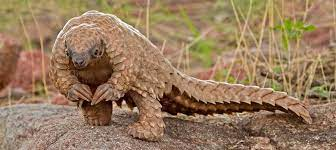
\includegraphics[]{pangolinpicture.jpg}
\end{frame}

\begin{frame}{A Picture of a Dachshund}
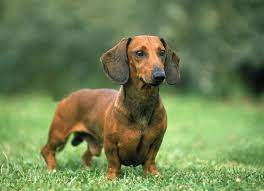
\includegraphics[]{wienerdog.jpg}
\end{frame}




\section{My Favorite Plot}

\begin{frame}[fragile]{Slide with R Code}
\begin{knitrout}
\definecolor{shadecolor}{rgb}{0.969, 0.969, 0.969}\color{fgcolor}\begin{kframe}
\begin{alltt}
\hlcom{# load in the data set}
\hlkwd{data}\hlstd{(penguins,} \hlkwc{package} \hlstd{=} \hlstr{"palmerpenguins"}\hlstd{)}
\hlkwd{head}\hlstd{(penguins)}
\end{alltt}
\begin{verbatim}
## # A tibble: 6 x 8
##   species island    bill_length_mm bill_depth_mm flipper_l~1 body_~2 sex    year
##   <fct>   <fct>              <dbl>         <dbl>       <int>   <int> <fct> <int>
## 1 Adelie  Torgersen           39.1          18.7         181    3750 male   2007
## 2 Adelie  Torgersen           39.5          17.4         186    3800 fema~  2007
## 3 Adelie  Torgersen           40.3          18           195    3250 fema~  2007
## 4 Adelie  Torgersen           NA            NA            NA      NA <NA>   2007
## 5 Adelie  Torgersen           36.7          19.3         193    3450 fema~  2007
## 6 Adelie  Torgersen           39.3          20.6         190    3650 male   2007
## # ... with abbreviated variable names 1: flipper_length_mm, 2: body_mass_g
\end{verbatim}
\begin{alltt}
\hlkwd{library}\hlstd{(ggplot2)}
\end{alltt}


{\ttfamily\noindent\color{warningcolor}{\#\# Warning: package 'ggplot2' was built under R version 4.1.3}}\end{kframe}
\end{knitrout}
\end{frame}

\begin{frame}{Slide with My "Favorite Plot"}
\begin{knitrout}
\definecolor{shadecolor}{rgb}{0.969, 0.969, 0.969}\color{fgcolor}\begin{kframe}


{\ttfamily\noindent\color{warningcolor}{\#\# Warning: Removed 2 rows containing missing values (`geom\_point()`).}}\end{kframe}\begin{figure}
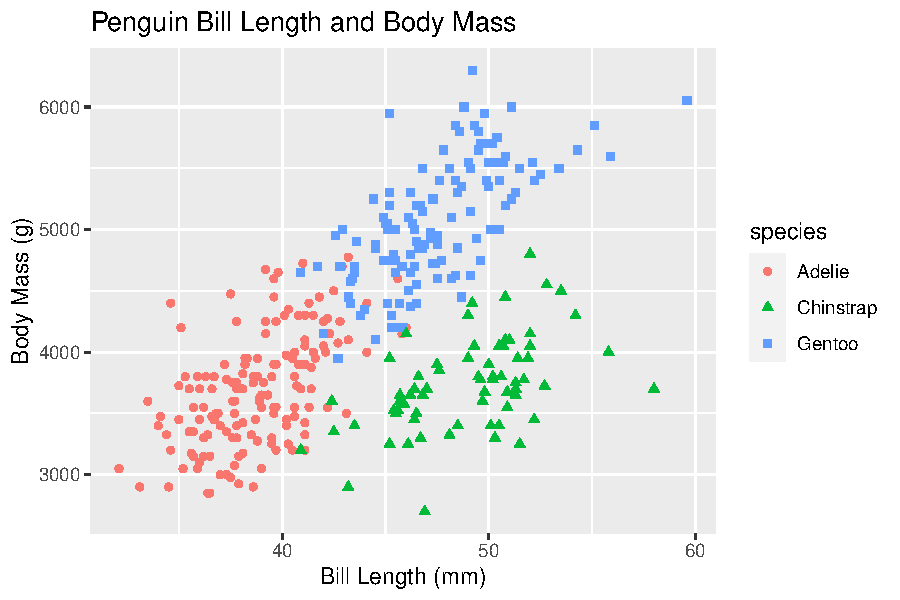
\includegraphics[width=\maxwidth]{figure/figure1-1} \caption[A test plot]{A test plot}\label{fig:figure1}
\end{figure}

\end{knitrout}
\end{frame}


\section{Link to my CV}

\begin{frame}{A link to the CV is provided below:}

\href{https://www.overleaf.com/project/636d4fd7bcff6d8a03449fde}{\beamergotobutton{Link}}

\href{Resume_CV_.pdf}{\beamergotobutton{Link}}


\end{frame}

\end{document}
